\documentclass[10pt,twocolumn,letterpaper]{article}

\usepackage{cvpr}
\usepackage{times}
\usepackage{epsfig}
\usepackage{graphicx}
\usepackage{amsmath}
\usepackage{amssymb}
\usepackage{caption}
\usepackage{subfig}
\usepackage{algorithm2e}

\graphicspath{ {img/} }

% Include other packages here, before hyperref.

% If you comment hyperref and then uncomment it, you should delete
% egpaper.aux before re-running latex.  (Or just hit 'q' on the first latex
% run, let it finish, and you should be clear).
\usepackage[breaklinks=true,bookmarks=false]{hyperref}

\cvprfinalcopy % *** Uncomment this line for the final submission

\def\cvprPaperID{****} % *** Enter the CVPR Paper ID here
\def\httilde{\mbox{\tt\raisebox{-.5ex}{\symbol{126}}}}

% Pages are numbered in submission mode, and unnumbered in camera-ready
%\ifcvprfinal\pagestyle{empty}\fi
\setcounter{page}{1}
\begin{document}

%%%%%%%%% TITLE
\title{Sequential and Parallel RGB Image Histogram Equalization in C++, OpenMP and CUDA}

\author{Alessandro Minervini\\
Matricola - 6414770\\
{\tt\small alessandro.minervini@stud.unifi.it}
% For a paper whose authors are all at the same institution,
% omit the following lines up until the closing ``}''.
% Additional authors and addresses can be added with ``\and'',
% just like the second author.
% To save space, use either the email address or home page, not both
\and
Francesco Lombardi\\
Matricola - 6344416\\
{\tt\small francesco.lombardi3@stud.unifi.it}
}

\maketitle
%\thispagestyle{empty}

%%%%%%%%% ABSTRACT
\begin{abstract}
	This work is about the implementation of an important task in Image Processing that makes clearer the vision of an image and homogeneous its histogram: Histogram Equalization.This technique has been applied to RGB images.The task has been realized in both sequential and parallel version, respectively in C++ and OpenMP/CUDA languages. Sequential and OpenMP ones have been tested on a machine having Intel core i5, dual core. Instead, CUDA code has been ran on a NVDIA Titan-X GPU, having 12Gb of RAM e 3072 CUDA cores.Performances have been finally evaluated in terms of speedup and curves representing the execution times to compute equalized images.
\end{abstract}

%%%%%%%%% BODY TEXT
\section{Introduction}
Images quality improvement is a very precious objective in Image Processing, which can be often achieved combining various techniques, for example Histogram Equalization.The procedure is based on computing the histogram of a grayscale image and modifying it in order to make it more homogeneous, the image clearer and brighter (if possible), and finally mapping old grey levels in new ones represented by the equalized histogram.

\subsection{Greyscale Images Histogram Equalization}
Image histogram represents the occurrence frequency of different color intensities in the image itself: it shows how many pixels of every possible color there are in the image. Every bin on the image histogram represents one intensity level, from 0 (black) to 255 (white). 

Histogram equalization usually increases the global contrast of an image, especially when it is represented by close contrast values. Through this adjustment, the intensities can be better distributed on the histogram. This allows for areas of lower local contrast to gain a higher one, highlights the gap through image foreground and other ones, underlines not explicit edges and contours. Histogram equalization accomplishes this by effectively spreading out the most frequent intensity values, thus obtaining a more homogeneous histogram. An application example for a greyscale image is shown below:

\begin{figure}[h]
	\centering
	\subfloat[Original Image]{{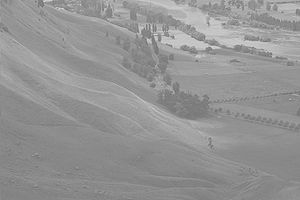
\includegraphics[width=3.7cm, height=3cm]{hill} }}
	\qquad
	\subfloat[Equalized Image]{{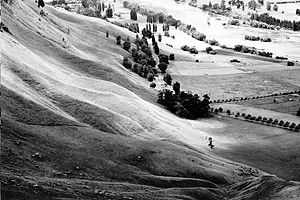
\includegraphics[width=3.7cm, height=3cm]{hill_eq} }}
	\qquad

	\subfloat[Original Histogram]{{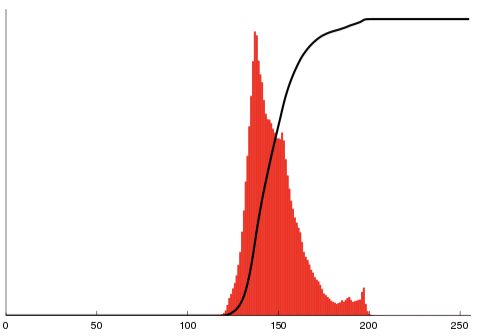
\includegraphics[width=3.7cm, height=3cm]{hist} }}
	\qquad
	\subfloat[Equalized Histogram]{{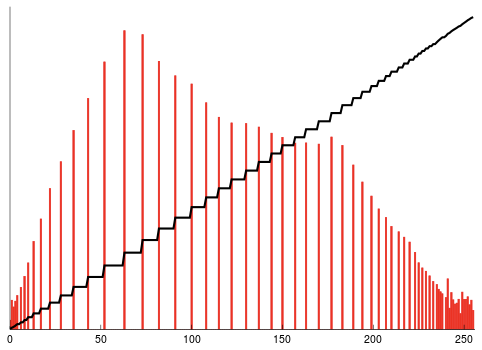
\includegraphics[width=3.7cm, height=3cm]{hist_eq} }}
	\caption{Histogram Equalization for a greyscale image.}
	\label{fig:grey_eq}
	
\end{figure}

\subsection{Theoretical Formulation}
Let \textit{f} be a given image represented as a NxM matrix of integer pixel intensities ranging from 0 to L-1 (255 in our case) and \textit{hist} the relative histogram.
The function ${h_{eq}}$ that equalizes this histogram is:

\begin{equation}
	h_{eq}(hist) =  round(\frac{cdf(hist) - cdf(0)}{(N * M) - 1} * (L - 1))
	\label{equalization}
\end{equation}

where ${cdf(hist)}$ is the cumulative distribution function of image histogram.

After equalization, each value of the original histogram is changed to the equalized one's, thus obtaining the equalized image.

\subsection{RGB Images Histogram Equalization}
The procedure we have analyzed so far has been applied also to a different class of images: RGB ones.The idea was born from a simple concept, which is the fact that, as in greyscale images we build an histogram representing pixel's intensities, we can do the same for 3 channel images (e.g. RGB). In order to do this, a color space switch is needed, because the equalization has to be done on the histogram representing image's brightness channel: we have chosen YUV space. So the first step we have made has been RGB to YUV image conversion, which can be defined as follows: \\
\\
	$\begin{cases} 
	Y = R * 0.299 + G * 0.587 + B * 0.114 \\
	U = R * -0.168736 + G * -0.331264 + B * 0.5 + 128 \\
	V = R * 0.5 + G * -0.418688 + B * -0.081312 + 128
	\end{cases}$\\
\\
The effect of this operation is shown in Figure \ref{fig:YUV}.

\begin{figure}[h]
	\centering
	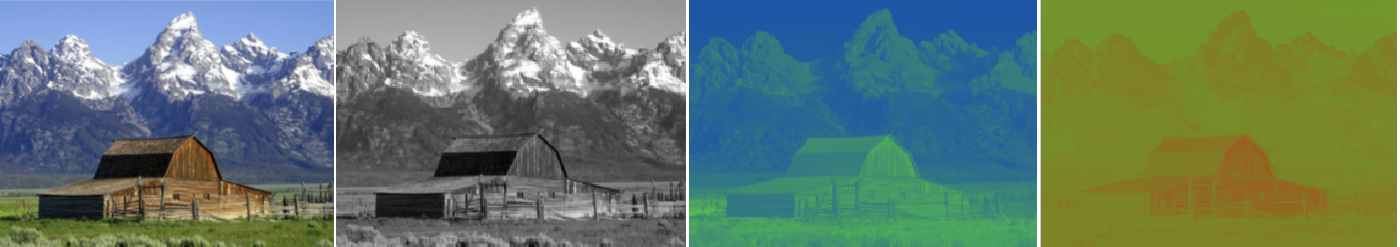
\includegraphics[width=8cm, height=2cm]{YUV}
	\caption{RGB to YUV Conversion}
	\label{fig:YUV}
\end{figure}

After this conversion the equalization has been applied to Y channel histogram, leaving U and V ones intact, and after that image has been reconverted to RGB, using the following equations:\\
\\
$\begin{cases} 
R = Y + 1.4075 * (V - 128)\\
G = Y - 0.3455 * (U - 128) - (0.7169 * (V - 128))\\
B = Y + 1.779 * (U - 128)
\end{cases}$\\
\\
The final result is shown in Figure \ref{fig:RGB_eq}.

\begin{figure}[h]
	\centering
	\subfloat[Original Image]{{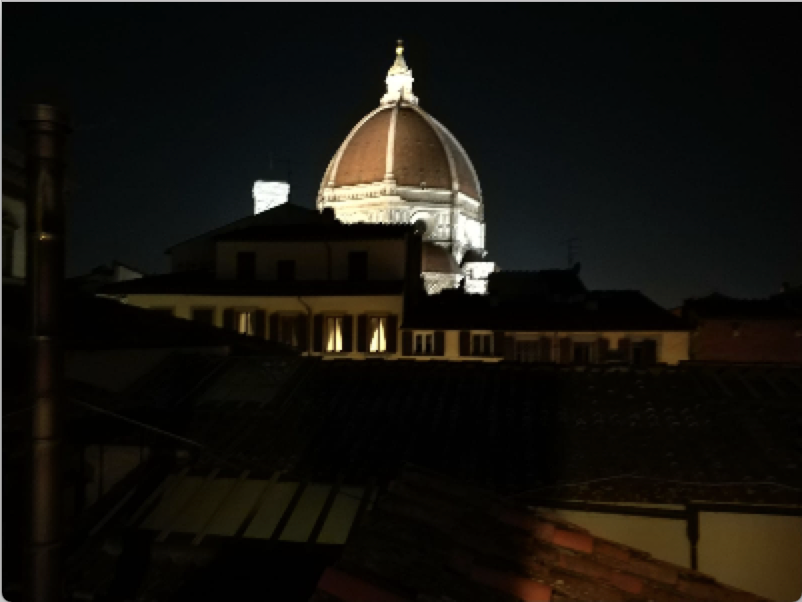
\includegraphics[width=3.7cm, height=3.7cm]{duomo} }}
	\qquad
	\subfloat[Equalized Image]{{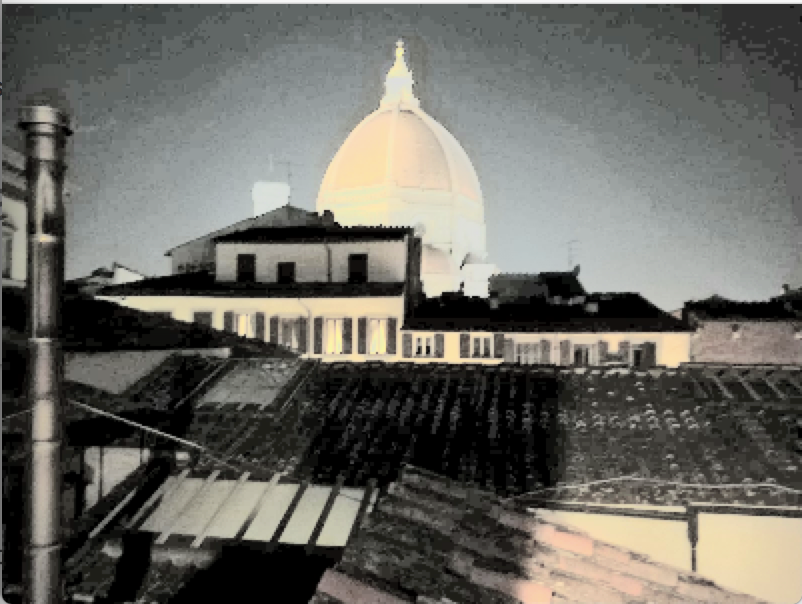
\includegraphics[width=3.7cm, height=3.7cm]{duomo_eq} }}
	\caption{RGB Equalized Image}
	\label{fig:RGB_eq}
\end{figure}

\section{Implementation}
\subsection{Sequential Version}
We have implemented the procedure described above through 3 functions (called in the following order): \textit{make histogram}, \textit{cumulative\_histogram} and \textit{equalize}.
The first one receives the image histogram as formal parameter and computes the RGB to YUV conversion, updating the Y histogram. The second function computes the cumulative distribution function and makes the equalization applying \ref{equalization}. The third one implements the conversion from YUV back to RGB image. The pseudo-code is the following:


\begin{algorithm}[h]
	\textbf{function Make\_Histogram}
	
	\KwData{image, histogram, YUV\_image\;}

	initialize histogram\;
	\For{i $=$ 0, i$\textless$image.cols, i $++$}{
		\For{j $=$ 0, j$\textless$image.cols, j $++$}{
			R, G, B = image(i,j)\;
			
			Y = R * 0.299 + G * 0.587 + B * 0.114\;
			
			U = R * -0.168736 + G * -0.331264 + B * 0.5 + 128\;
			
			V = R * 0.5 + G * -0.418688 + B * -0.081312 + 128\;
			
			histogram[Y]++\;
			
			YUV\_image(i,j) = Y, U, V\;
		}
	}
	\caption{Make\_histogram}
\end{algorithm}

\begin{algorithm}[h]
	\textbf{function Cumulative\_Histogram}
	
	\KwData{histogram, equalized\_histogram, image.cols, image.rows\;}
	
	cumulative\_histogram[256]\;
	
	\For{i $=$ 0, i$\textless$256, i $++$}{
		cumulative\_histogram[i] = histogram[i] + cumulative\_histogram[i-1]\;
		equalized\_histogram[i] = (cumulative\_histogram[i] - histogram[0])/(cols * rows - 1)*255)\;
	}
	\caption{Cumulative\_histogram}
\end{algorithm}

\newpage

\begin{algorithm}[h]
	\textbf{function Equalize}
	
	\KwData{image, equalized\_histogram, YUV\_image\;}
	
	initialize histogram\;
	\For{i $=$ 0, i $\textless$ image.cols, i $++$}{
		\For{j $=$ 0, j $\textless$ image.cols, j $++$}{
			Y = equalized\_histogram[YUV\_image(i,j)]\;
			U = YUV\_image(i,j)\;
			V = YUV\_image(i,j)\;
			
			R = max(0, min(255,(int)(Y + 1.4075 * (V - 128))))\;
			G = max(0, min(255,(int)(Y - 0.3455 * (U - 128) - (0.7169 * (V - 128)))))\;
			B = max(0, min(255,(int)(Y + 1.7790 * (U - 128))))\;
			
			image(i,j) = R, G, B\;
		}
	}
	\caption{Equalize}
\end{algorithm}

\subsection{Parallel versions}

\subsubsection{OpenMP Parallel Version}
The first technology used to parallelize the procedure above is OpenMP, an API which supports multi-platform shared memory multiprocessing programming in C, C++ and Fortran. 

The OpenMP parallel version of the code is implemented as the sequential one, with the main difference that, as OpenMP rules, the same functions implemented in the sequential version have been written into a particular OMP structure that parallelizes the sequential for loops: \textit{\#pragma omp parallel for}. The use of this structure has been really easy and convenient: in fact it is made in such a way as to decide the number of threads to be used, depending on the task to execute and the machine which runs it.

\subsubsection{CUDA Parallel Version}
The second technology used to parallelize Histogram Equalization is CUDA, a parallel computing platform and application programming interface (API) model created by Nvidia. It allows to use a CUDA-enabled GPU for general purpose processing. The platform is designed to work with programming languages such as C, C++, and Fortran. For this project we ran CUDA code on a NVDIA Titan-X GPU.

The main idea for task's parallelization has been the following: if possible, depending on the number of CUDA cores, pixels of the image have been processed one per thread. Otherwise what happens is illustrated in Figure \ref{fig:shared}.

\begin{figure}[h]
	\centering
	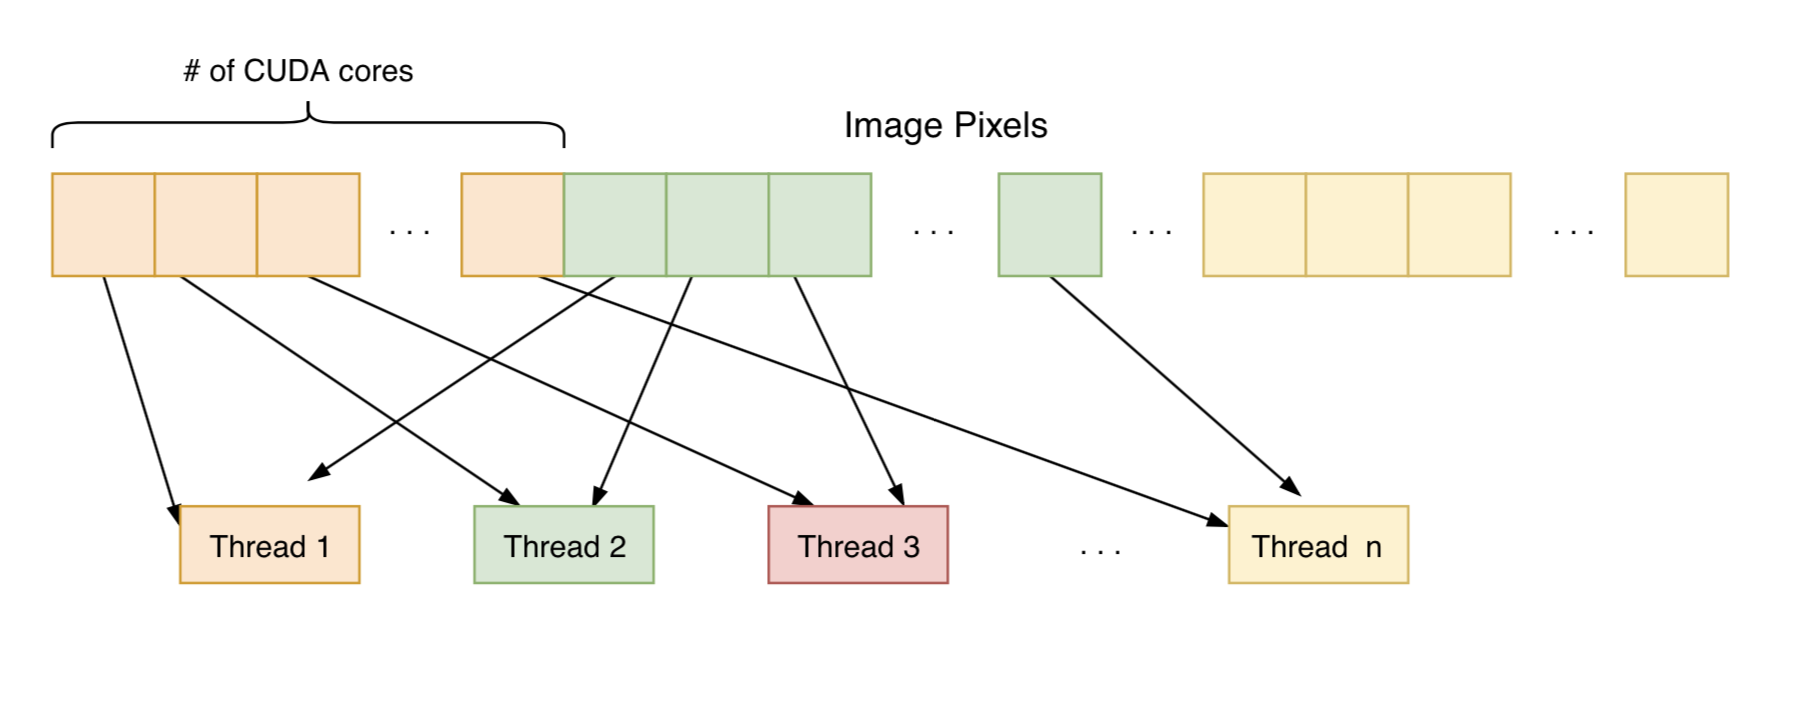
\includegraphics[width=8.5cm, height=4cm]{shared}
	\caption{CUDA image management}
	\label{fig:shared}
\end{figure}

A special zoom has to be done on GPU management: we have allocated a char array to represent the image and three int[256] arrays in order to store image histogram, image equalized histogram and the cumulative distribution function. After that we have copied them from the host (CPU) to the device (GPU) through the function \textit{cudaMemCpy}. Next, the functions illustrated in sequential version have been reproduced as three CUDA kernels: \textit{make\_histogram}, \textit{equalize} and \textit{YUV2RGB}: they have been called in the same order as before, computing the equalization. Finally we have freed the GPU through the function \textit{cudaFree} and saved the results.

\section{Results}
Tests have been performed using the same set of images, from 100x100px to 12800x12800px in 8 width x height steps obtained doubling these dimensions iteratively. All results have been achieved mediating over 10 run. They have also been evaluated when varying the number of threads until saturation (relatively to the machine used for testing). 

With OpenMP version we have tested the images above with 2, 4 and 8 threads, with the following result:
%immagine OMP
\begin{figure}[h]
	\centering
	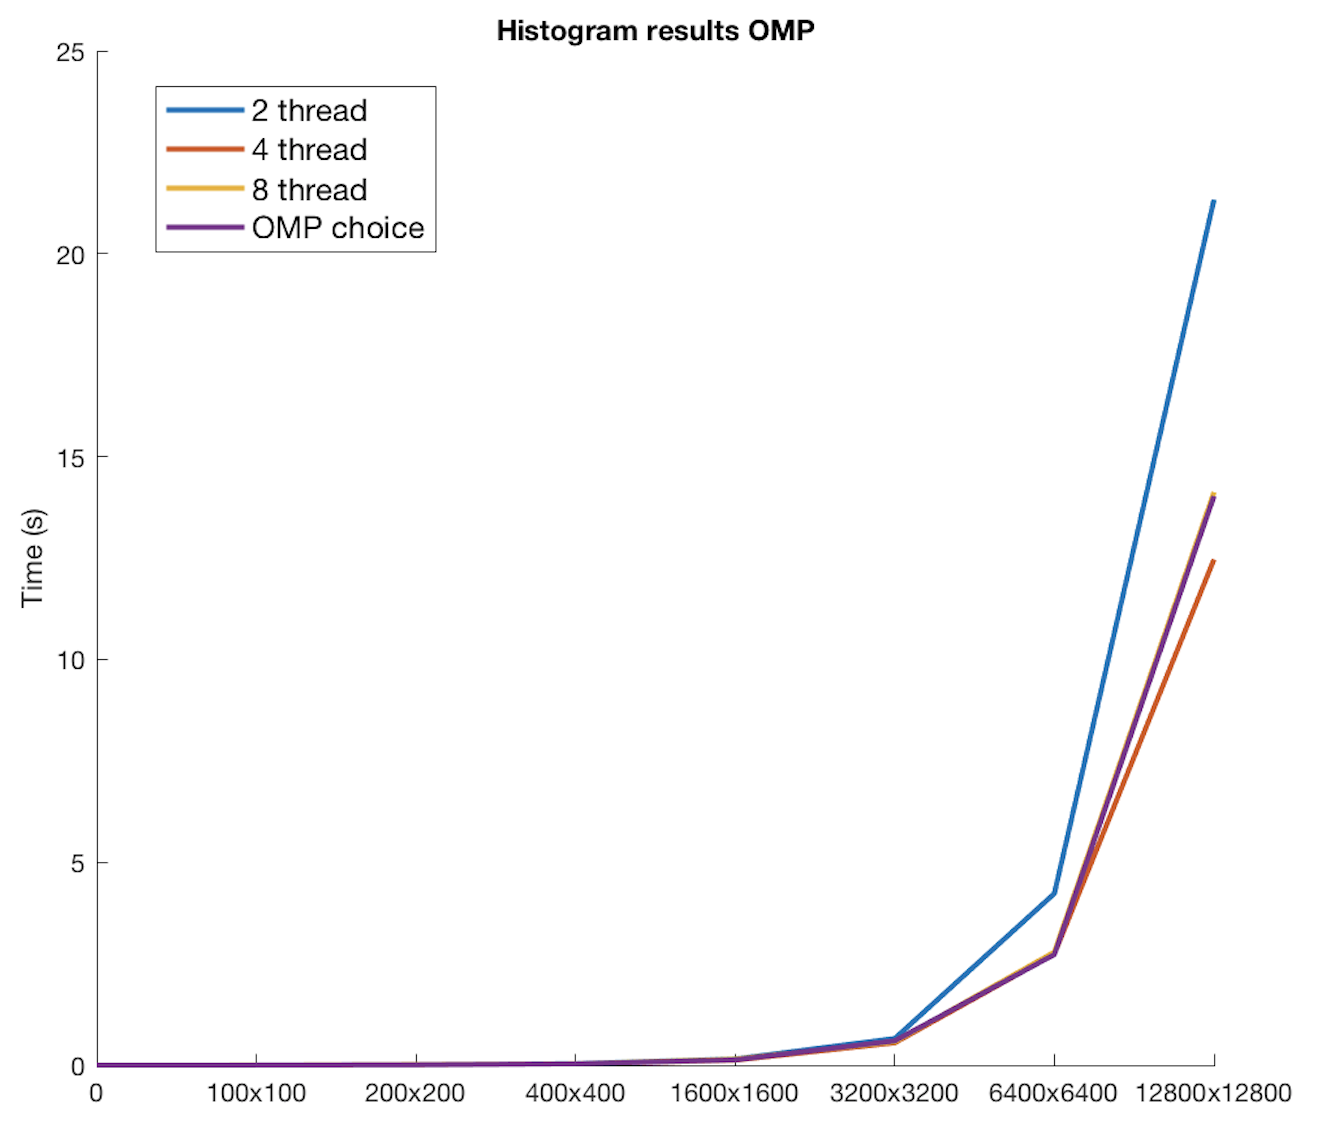
\includegraphics[width=8cm, height=7cm]{res_OMP}
	\caption{OpenMP results}
	\label{fig:OMP}
\end{figure}

How about CUDA code, we have evaluated that the best configuration was the one described before (1 CUDA core per pixel), and we report the curve representing relative results:
%immagine CUDA
\begin{figure}[h]
	\centering
	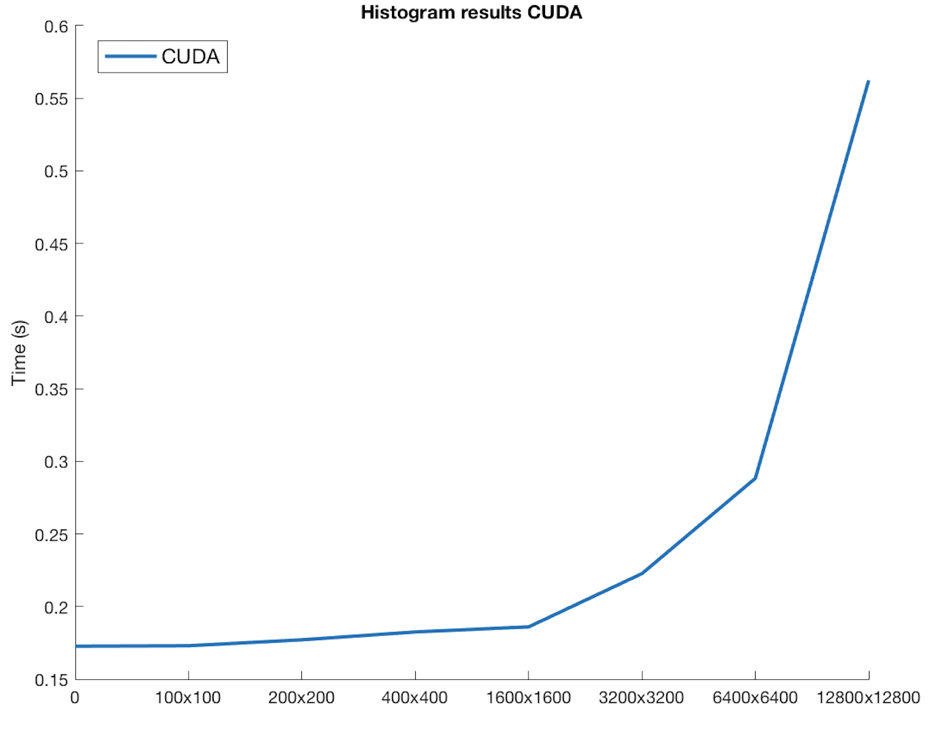
\includegraphics[width=8cm, height=7cm]{res_CUDA}
	\caption{CUDA results}
	\label{fig:CUDA}
\end{figure}

As final result we report in Figure \ref{fig:global}  a global evaluation of each version's best configuration.
%immagine globale
\begin{figure}[h]
	\centering
	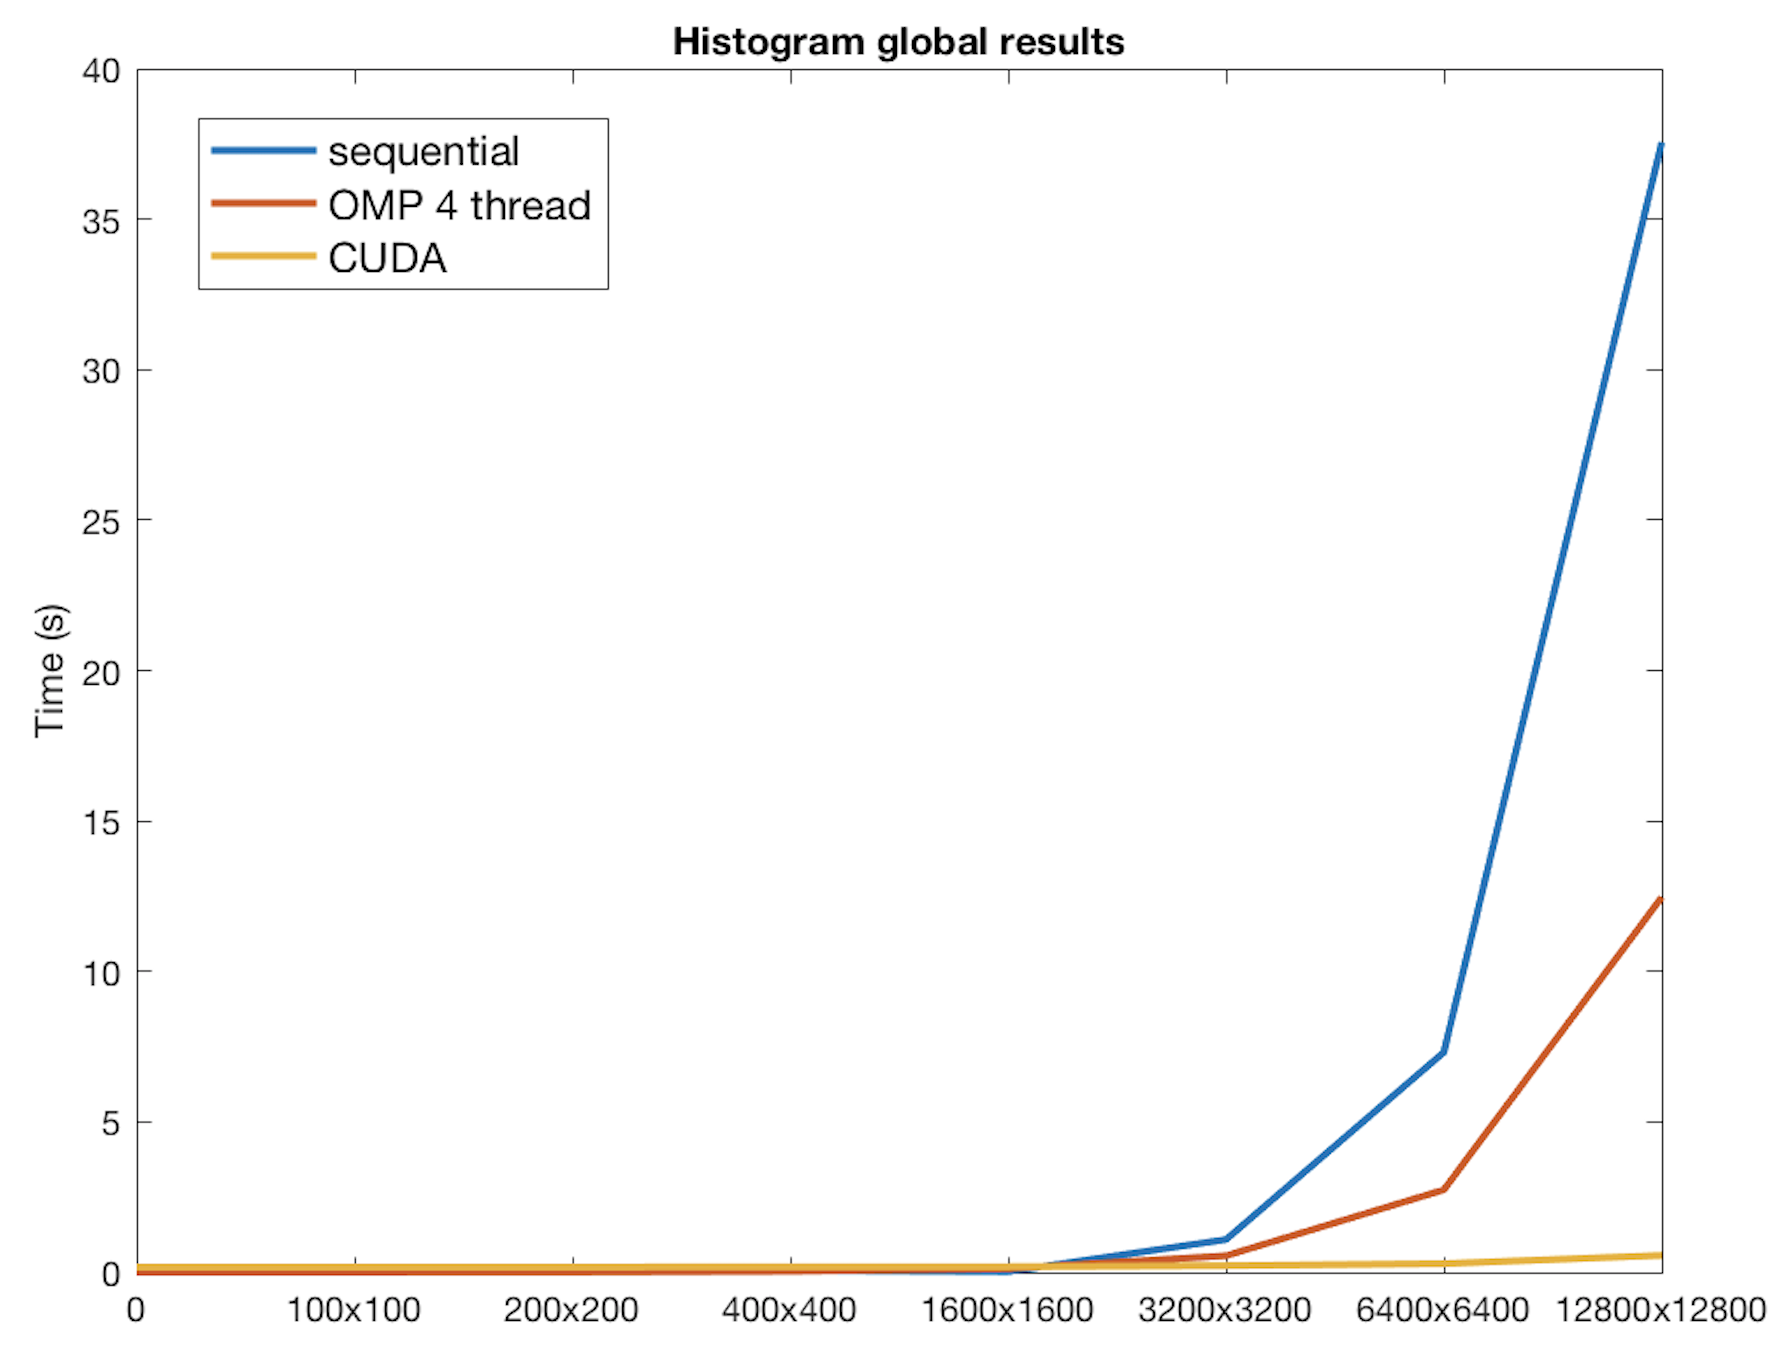
\includegraphics[width=8cm, height=7cm]{res_global}
	\caption{Final Results}
	\label{fig:global}
\end{figure}


\subsection{Speed Up}
The following figures represents the speed-up obtained with OpenMP and CUDA against sequential implementation.
%immagine con i 2 speed up
\begin{figure}[h]
	\centering
	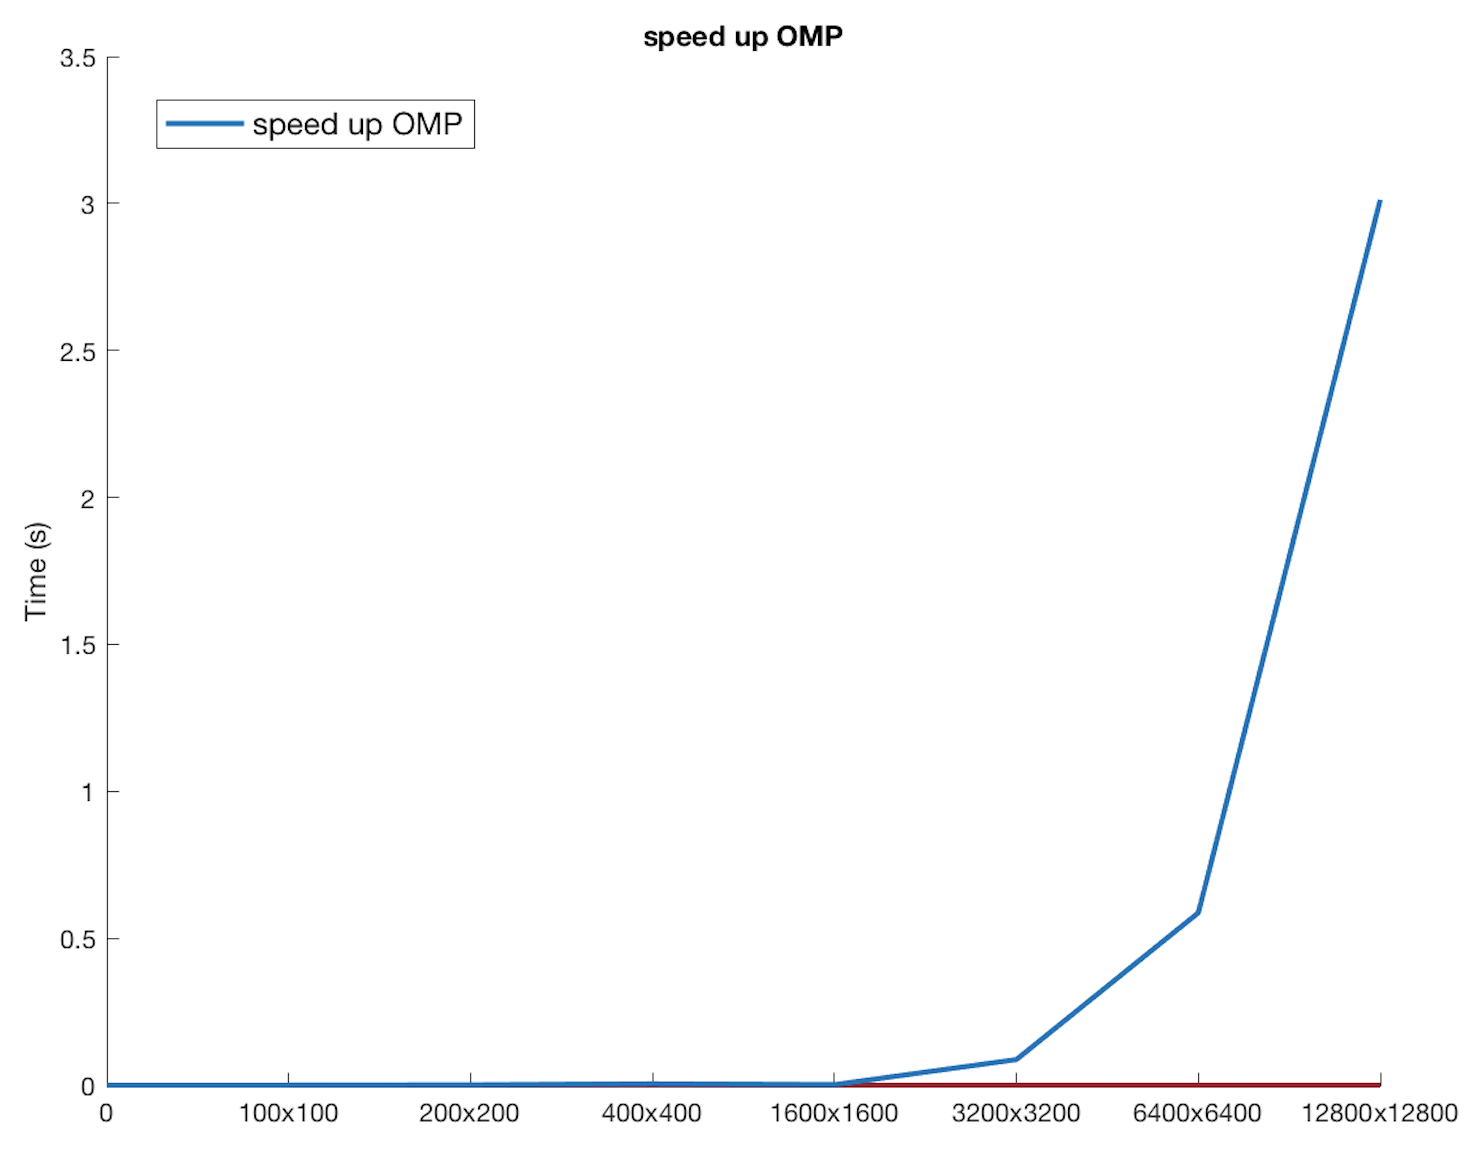
\includegraphics[width=8cm, height=6cm]{speed_up_OMP}
	\caption{Speed up OMP}
	\label{fig:s-u-omp}
\end{figure}

\begin{figure}[h]
	\centering
	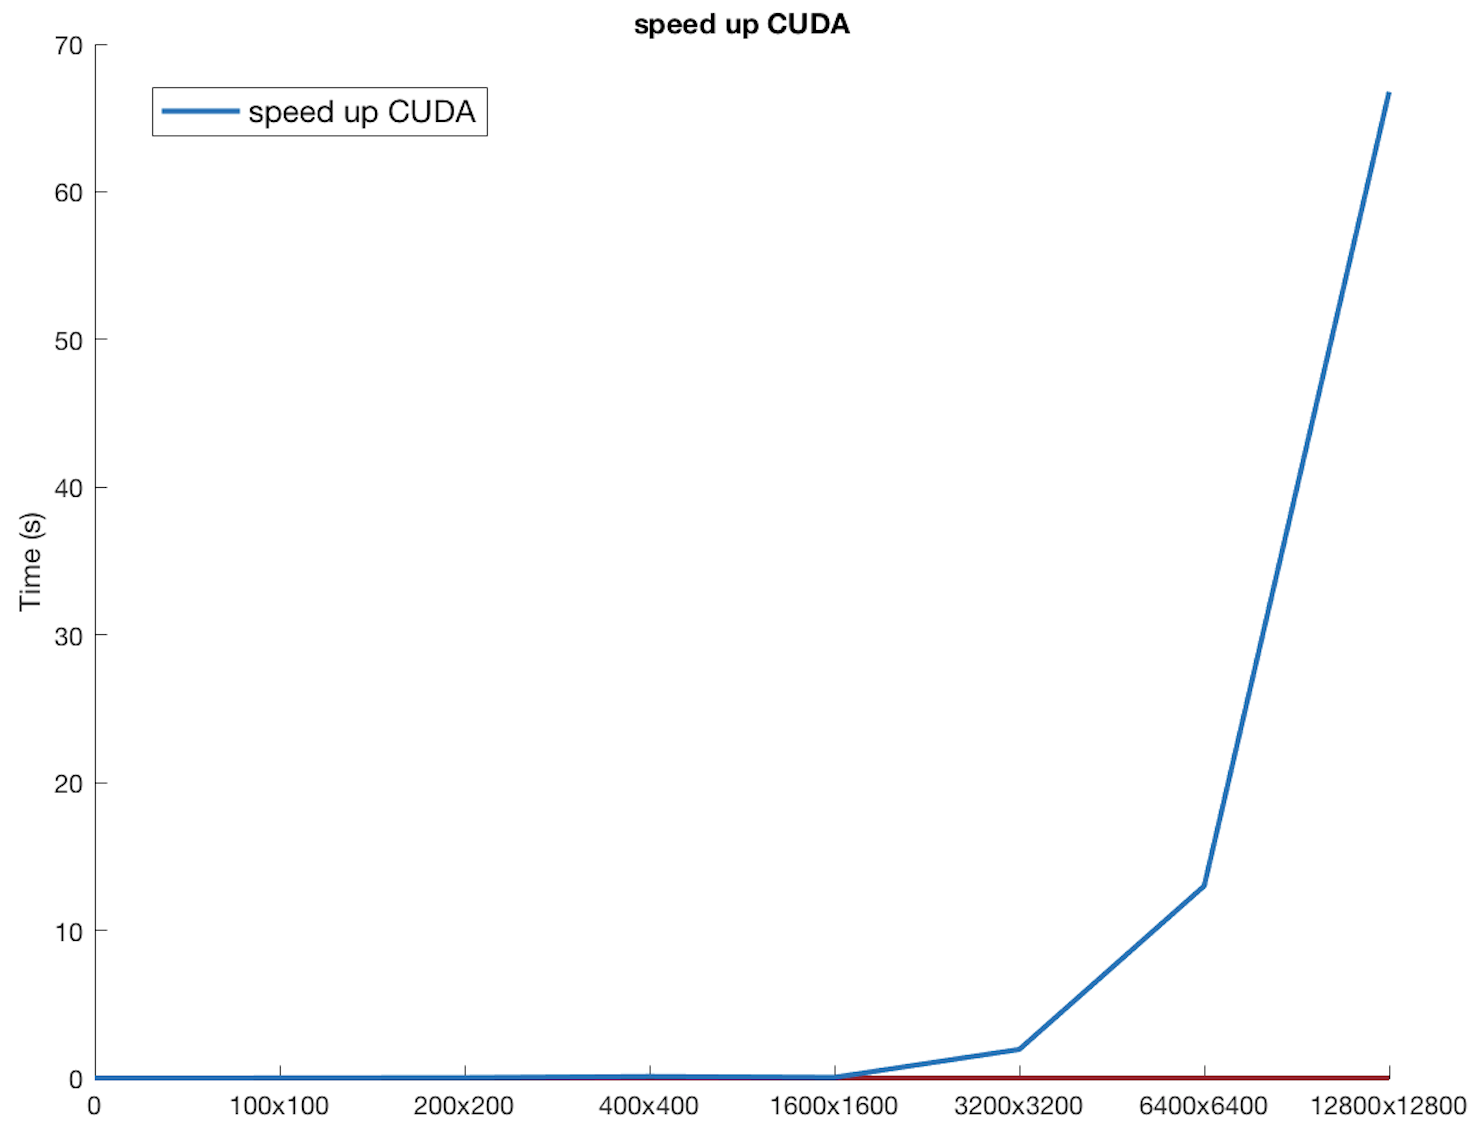
\includegraphics[width=8cm, height=6cm]{speed_up_CUDA}
	\caption{Speed up CUDA}
	\label{fig:s-u-CUDA}
\end{figure}

\begin{figure}[h]
	\centering
	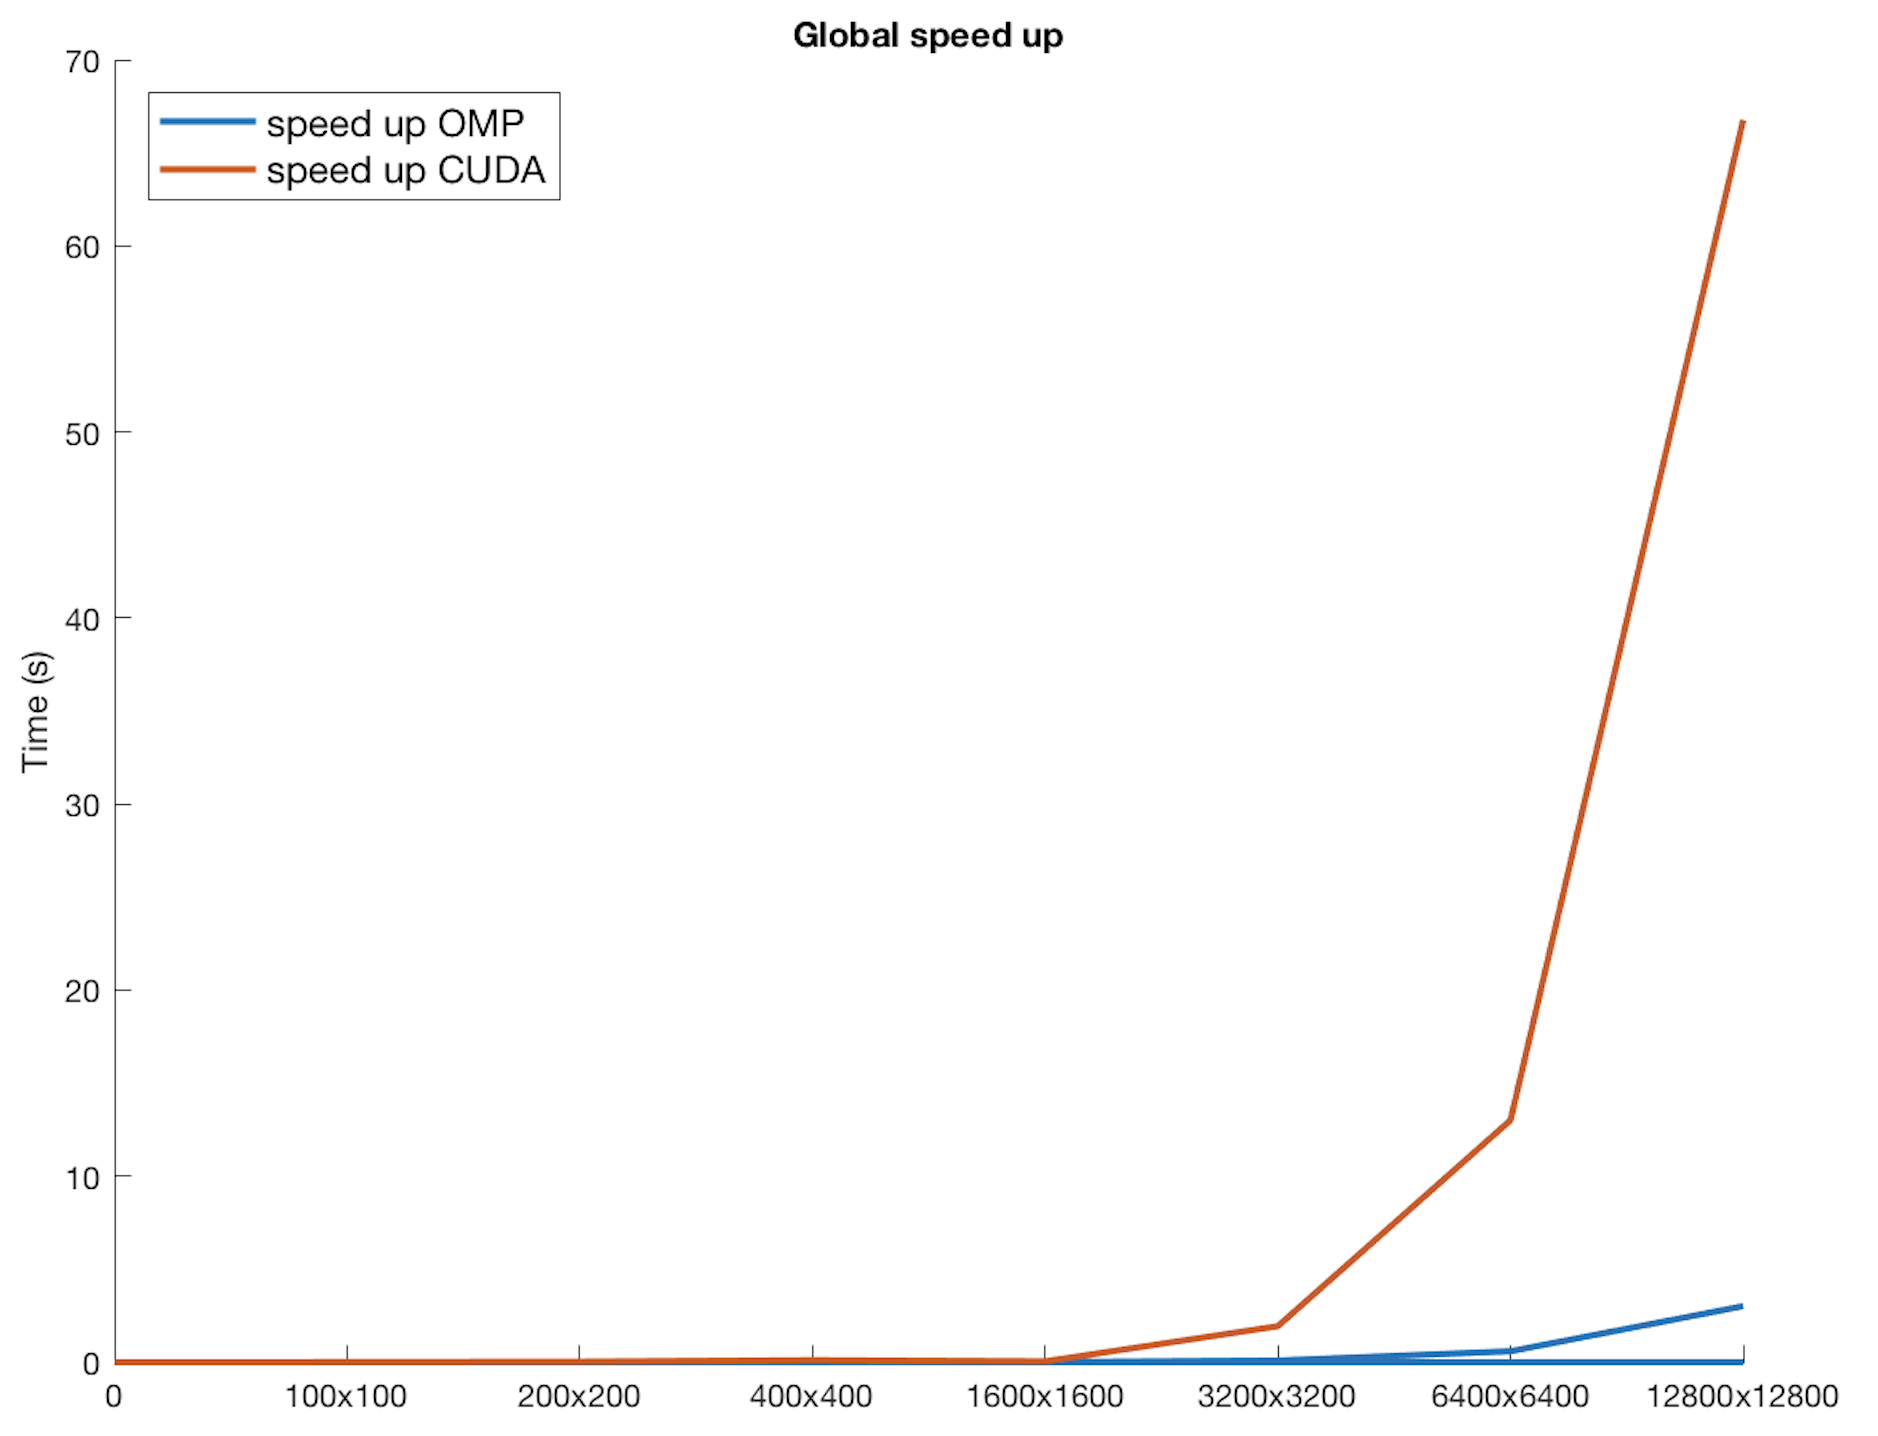
\includegraphics[width=8cm, height=6cm]{global_speed_up}
	\caption{Global Speed Up}
	\label{fig:glob-s-u}
\end{figure}

\section{Notes}
OpenCV library has been used to load, resize and (in CUDA) save images.

Two different time evaluators have been used to compute execution time:
	\begin{itemize}
		\item OpenMP's  \textit{omp\_get\_wtime()} for sequential and OMP versions;
		\item \textit{gettimeofday()} for CUDA version;
	\end{itemize}

\end{document}
